%TITLE, AUTHOR, DATE
\documentclass[12pt, a4paper]{article} %14 pt indicates the font size of the prepared document
\usepackage[margin=1in]{geometry}
\usepackage[utf8]{inputenc}
\usepackage{multicol}
\usepackage{multirow}
\usepackage{color}
\usepackage{enumerate}
\usepackage{amsmath}
\usepackage{graphicx}
\usepackage{calligra}
\usepackage{hyperref}
\usepackage{subcaption}
\usepackage{biblatex}
\addbibresource{bibfile.bib}

\title{CSE 300: Online Assignment}
\author{Md Shamsuzzoha Bayzid$^{1,\dagger}$, Mahjabin Nahar$^{1}$, Md Shariful Islam\\ Bhuyan$^{1}$, and Md Saidur Rahman$^{1}$ \\ \\
	$^1$Department of Computer Science and Engineering \\
	Bangladesh University of Engineering and Technology \\
	*Corresponding author: shams bayzid@cse.buet.ac.bd \\
	These authors contributed equally to this work
}
\date{April 2021}

\begin{document}
	\maketitle
	
	\section{Graphics}
Emacs, Nano, or Vim: Choose your Terminal-Based Text Editor Wisely. Nano
is the built-in basic text editor for many popular distros. Its usually already
contained in the distro, doesnt take any learning or getting used to, and all
its commands and prompts are displayed at the bottom. Nano is the built-in
basic text editor for many popular distros. Its usually already contained in the
distro, doesnt take any learning or getting used to, and all its commands and
prompts are displayed at the bottom. Vi or one of its variants typically comes
with your distro-of-choice. Its considered a modal editor, which means there
are different modes for navigating files and editing text. Because you navigate
Vi most efficiently through the use of keyboard commands and shortcuts, Vi is
better experienced than explained.


	\begin{figure}[h!]
	\begin{subfigure}{.33\textwidth}
		\centering
		
\includegraphics[width=.4\linewidth]{emacslogo.png}
		\caption{emacs}
		\label{fig:sfig1}
	\end{subfigure}%
	\begin{subfigure}{.33\textwidth}
		\centering
		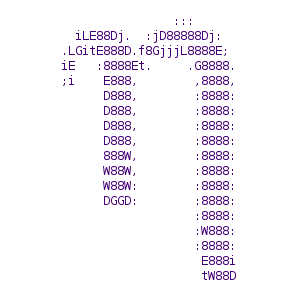
\includegraphics[width=.4\linewidth]{nanologo.png}
		\caption{nano}
		\label{fig:sfig2}
	\end{subfigure}
	\begin{subfigure}{.33\textwidth}
		\centering
		
\includegraphics[width=.4\linewidth]{vimlogo.png}
		\caption{nano}
		\label{fig:sfig2}
	\end{subfigure}
\caption{ Terminal-based text-editors
}
\end{figure}

\section{Equations}
In algebra, a quadratic equation is any equation having the form $ax2 +bx+c = 0$
where x represents an unknown, and a, b, and c represent known numbers, with
$a \neq 0$. It can easily be seen, by polynomial expansion, that the following
equation is equivalent to the quadratic equation:
$$\left(x+\frac{b}{2}\right)^2 = \frac{b^2 - 4ac}{4a^2}$$

$$x = \frac{-b + \sqrt{b^2 - 4ac}}{2a}$$

$$f_1(t) = \int_{3}^{5}\sin (x)dx$$

$$F(x) = A_0 + \displaystyle\sum_{n=1}^{N}\left[A_n\cos \left(\frac{2\pi nx}{P}\right) + B_n\sin \left(\frac{2 \pi nx}{P} \right) \right]$$

$$\lim\limits_{x \to a}\frac{f(x)-f(a)}{x-a}$$

$$\binom{a}{b+c} \binom{\frac{n^2-1}{2}}{n+1}$$

$$h \leq \sqrt{\frac{(s-a)(s-b)(s-c)}{s}}$$
	
$$6CO_2 + 6H_2O = 6C_12H_22O_11 + 6H_2O$$	
	
$$
\left[
\begin{matrix}
	a_1 & a_2 & a_3\\
	b_1 & b_2 & b_3\\
	c_1 & c_2 & c_3\\
\end{matrix}
\right]
$$

$$
e^{i\theta} = \cos \theta + i\sin \theta 
$$
\begin{equation*}
	\begin{split} 
		e^{i\frac{\pi}{2}} &= \cos \frac{\pi}{2} + i\sin \frac{\pi}{2}\\
		& = 0 + i.1\\
		& = i
\end{split}		
\end{equation*}

$$
 {}^{n}C_{k} = {n \choose r} = \frac{n!}{(n-r)!}
$$

$$
F_c(x,y) = \begin{cases}
	\frac{\delta^2x^3y^x}{\delta x^2} + 
	\frac{\delta^2\Gamma(x)log(tan(y))}{\delta x\delta y} & 
	\text{if } x,y 
	\text{ are real numbers}\\
	\lim\limits_{z \to e^{x^{2y}}}\sqrt{z+\frac{1}{\sqrt{z+\frac{1}{\sqrt{z+\hdots}}}}}&
	
	\text{otherwise}\\
\end{cases}
$$


\section{Bibliography}
The recent success of neural networks has boosted research on pattern recog-
nition and data mining. Many machine learning tasks such as object detection
in “You Only Look Once” \cite{redmon2016you}, machine translation [4], and speech recognition
[1], which once heavily relied on handcrafted feature engineering to extract in-
formative feature sets, has recently been revolutionized by various end-to-end
deep learning paradigms, i.e., convolutional neural networks (CNNs) [3], long
shortterm memory (LSTM) [2], and autoencoders.

	

\printbibliography
\end{document}
